	
	\section{Setup}
	Damit alles funktioniert, musst du deine Geräte zuerst überprüfen und einrichten. Dabei lernst du, wie du die einzelnen Komponenten miteinander verbindest und neu erstellte Programme auf das Smartphone überträgst.
	Zuerst musst du dazu das Smartphone und den Roboter mit dem \textbf{USB-Kabel} verbinden. Überprüfe dabei ob
	\begin{itemize}
		\item Alle Kabel am Roboter ordentlich sitzen und
		\item Dein Smartphone entweder mit dem WLAN \bfcode{MD005-2.4GHz} oder \bfcode{MD0029-2.4GHz} verbunden ist.
	\end{itemize}
	\begin{minipage}{.8\textwidth}
		Nun kannst du den Roboter durch Drücken der Enter-Taste starten.
		Die Tastenbelegung kannst du im Anhang in Abbildung \ref{fig:buttons} auf Seite \pageref{fig:buttons} nachschauen. Während der Roboter startet, kannst du auch die Mindroid-App auf dem Handy starten.
		Du musst nicht warten bis der Roboter fertig gestartet ist.
	\end{minipage}
	\begin{minipage}{.19\textwidth}
	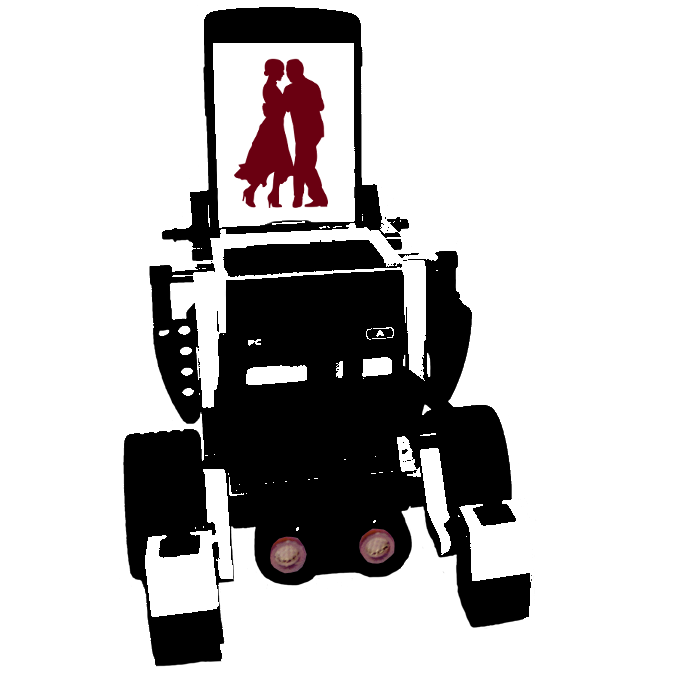
\includegraphics[width=\textwidth]{img/app_logo}	
	\end{minipage}
	
	\subsubsection{App und PC verbinden}
	Um neue Programme einfach und schnell auf das Smartphone übertragen zu können, muss zuerst das Smartphone mit dem PC verbunden werden. Dazu sind folgende Schritte nötig:
	\begin{enumerate}
	\begin{minipage}{.47\textwidth}	
	\item Starte den \textbf{Message-Server}, indem du die \textbf{ServerStarten.bat} auf dem Desktop des Computers mit einem Doppelklick ausführst. Der Server erledigt ein paar Einstellungen. Außerdem ist er später wichtig, damit die Roboter untereinander kommunizieren können.	 
	\item Um eine dauerhafte Verbindung herzustellen, müssen wir nun das Smartphone mit dem Server bekannt machen.	
	\item Der Message-Server zeigt dir links unten in der Ecke seine IP-Adresse an (siehe Screenshot auf Seit \pageref{fig:server}). Diese musst du nun der Mindroid-App mitteilen. Dazu navigierst du über das Menü oben links in den \textbf{Einstellungen-Bildschirm} (Abbildung rechts). Dort trägst du unter \textbf{MSG-Server IP} die IP des Servers ein. Ist dies erledigt, kannst du zurück zum Hauptbildschirm der App und auf \textbf{Verbinden} klicken. Die App verbindet sich nun mit dem Server.	
	\end{minipage}	
	\hfill
	\begin{minipage}{.47\textwidth}
	
	\centering
	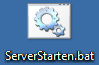
\includegraphics[width=.4\textwidth]{img/pc_serverbat.png}
	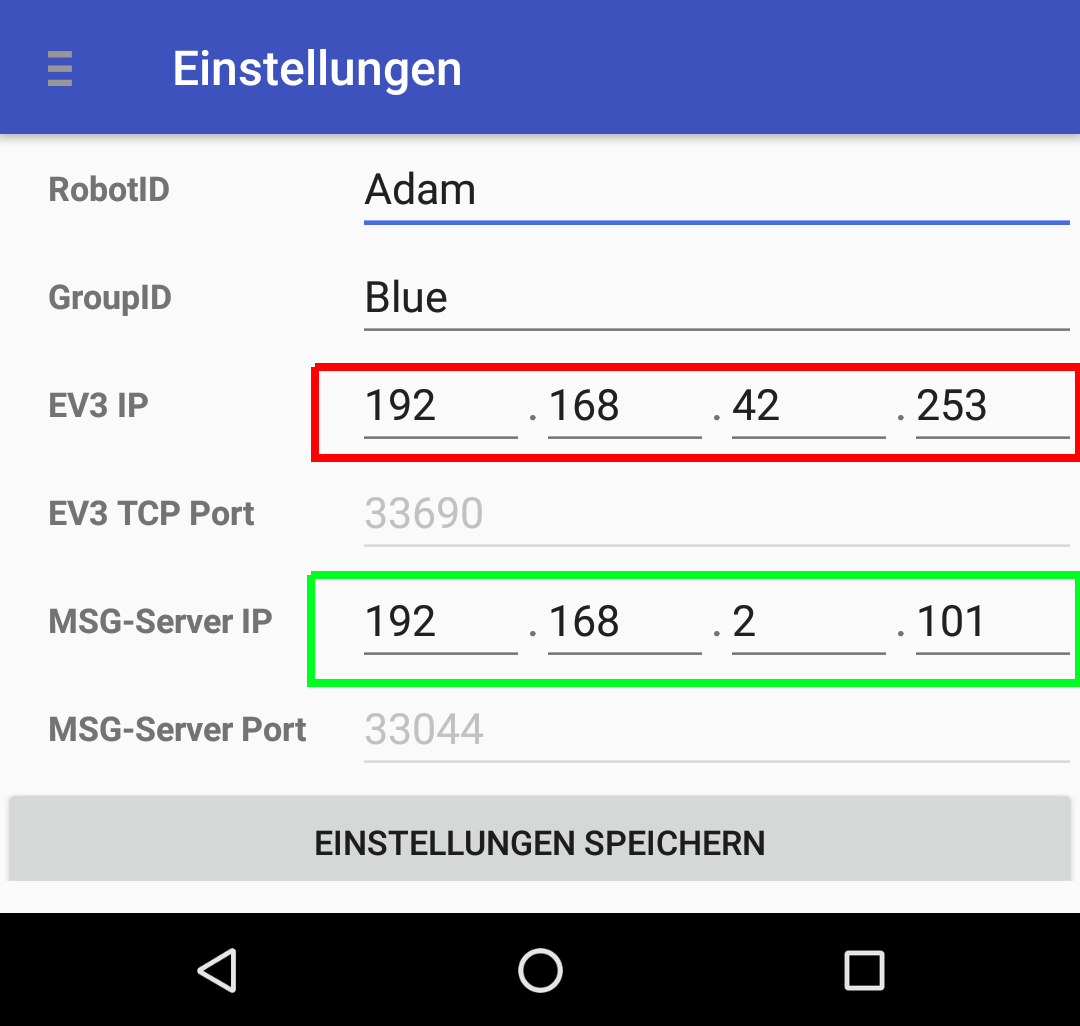
\includegraphics[width=.8\textwidth]{img/app_settings_short.png}
	\label{fig:app_settings}
	\end{minipage}
	\begin{center}
	\begin{figure}
	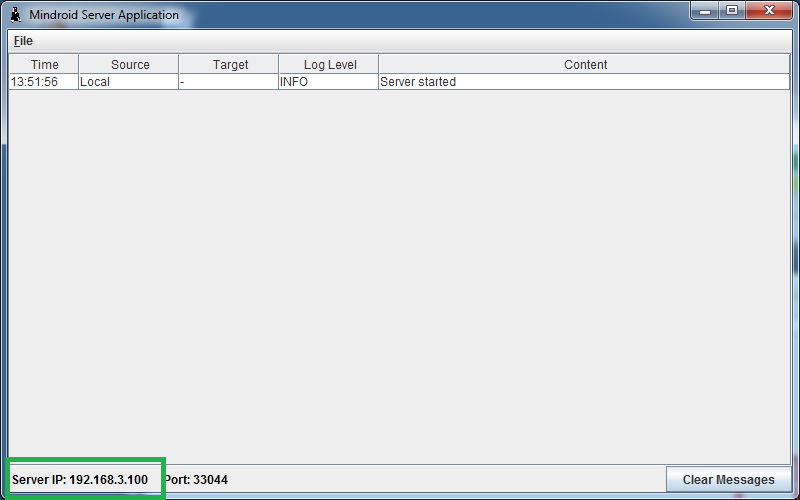
\includegraphics[width=.9\textwidth]{img/pc_server.png}
	\caption{Screenshot des Servers}
	\label{fig:server}
	\end{figure}
	
	\end{center}	

	
	
	\end{enumerate}
	
	\newpage
	
	
	\subsubsection{Programme übertragen}
	Neue Programme schreiben und übertragen wir in der	Enwicklungsumgebung \textbf{"Java-Editor"}.
	
	\begin{enumerate}
	\item Starte diesen indem du die Verknüpfung auf dem Desktop startest. In der Mitte findest du den Quelltext des aktuellen Programms, hinterlegt mit Farben, die die Orientierung erleichtern sollen.
	
	\gcenterone{img/je_main.png}
	
	Wie das Programm genau funktioniert, sehen wir uns gleich an. Zunächst einmal wollen wir es auf das Smartphone spielen, um zu sehen, was passiert.
	
	\item Dazu klickst du auf den blauen Play-Button oben links (Der Button ändert seine Farbe nach dem Durchlauf wieder zu türkis). 
	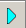
\includegraphics{img/je_playbutton.png} \\ Dein “Hallo Welt”-Programm wird jetzt an das Handy übertragen.
	
	\item In der Konsolenausgabe am unteren Bildrand sollte in etwa folgender Text erscheinen:
	\gcenterone{img/je_console.png}
	Das Programm ist nun übertragen.
	\end{enumerate}
	\newpage
	\subsubsection{Roboter und App verbinden}
	Zuletzt müssen nun noch Smartphone und Roboter miteinander verbunden werden. 
	
	
	\begin{enumerate}
	
	\begin{minipage}{.45\textwidth}
	\item Überprüfe dazu, ob wie rechts gezeigt die IP-Adresse 192.168.42.253 im Hauptmenü angezeigt wird. Ist dies nicht der Fall, folge der Anleitung in Abschnitt \ref{sec:pan} auf Seite \pageref{sec:pan}. 
	\end{minipage}
	\hfill	
	\begin{minipage}{.45\textwidth}
	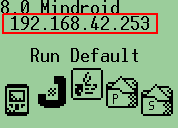
\includegraphics[width=.9\textwidth]{img/ev3_main.png}
	\end{minipage}
	
	\begin{minipage}{.45\textwidth}
	\item Wird die \textbf{IP-Adresse} im Hauptmenü des Roboters richtig angezeigt, musst du nun noch kontrollieren, ob diese IP-Adresse auch im Einstellungsmenü der App richtig gesetzt ist. Überprüfe dazu den Eintrag unter \textbf{EV3 IP}. Die farblichen Markierungen auf den Bildern sind dir dabei eine Hilfe. Falls der Eintrag nicht korrekt ist, korrigiere ihn.
	\end{minipage}	
	\hfill	
	\begin{minipage}{.45\textwidth}
	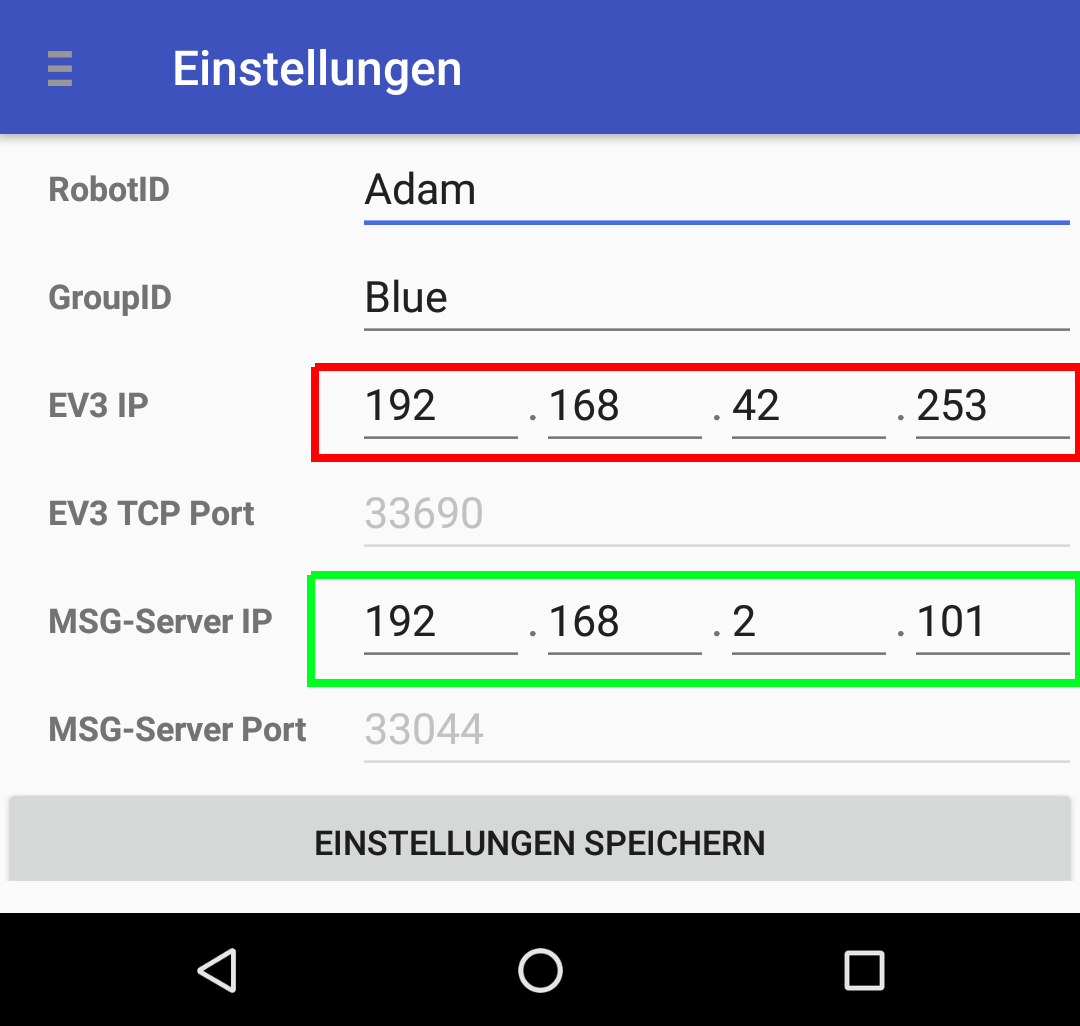
\includegraphics[width=.9\textwidth]{img/app_settings_short.png}
	\end{minipage}
	
	
	\item \label{sec:afterpan}Nun kannst du das \textbf{EV3-Programm }starten. Wähle dazu \textbf{Run Default} im Hauptmenü des Roboters aus und bestätige mit der Auswahltaste. Danach musst du warten, bis der Roboter \textbf{"Ready"} anzeigt
	
	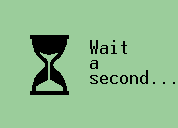
\includegraphics[width=.3\textwidth]{img/ev3_waitasecond.png}
	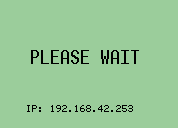
\includegraphics[width=.3\textwidth]{img/ev3_pleasewait.png}	
	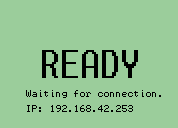
\includegraphics[width=.3\textwidth]{img/ev3_ready.png}
	\item Der Roboter ist nun bereit dazu sich mit dem Handy zu verbinden. In der App kannst du nun \glqq Verbindung zum EV3-Brick herstellen\grqq{} antippen.
	\item Um nun das Hello-World-Programm zu starten, wähle es in der Liste der App aus und drücke auf \textbf{Starten}. Es wird ausgeführt, und auf dem Bildschirm des Roboters erscheint \textbf{"Hallo Welt!"}
	
	\end{enumerate}	
	\newpage

		
	
	